\documentclass[a4paper,12pt,oneside,final]{extbook}

\usepackage[utf8]{inputenc}
\usepackage[T1]{fontenc}
\usepackage{graphicx}
\usepackage{times}
\usepackage[english,swedish]{babel}
\usepackage[export]{adjustbox}
\usepackage{geometry}
\usepackage{array}
\usepackage{float}
\usepackage{caption}

\geometry{
 margin=20mm
} 

\usepackage{fancyhdr}

\usepackage{titling}
\title{Individuell rapport, TNM094}
\author{Daniel Olsson\\Flerreglarsspel}

\frenchspacing
\setlength{\parindent}{0pt}
\parskip 5pt
\usepackage{lscape}
\usepackage{color}
\definecolor{rltred}{rgb}{.5,0,0}
\definecolor{rltgreen}{rgb}{0,.5,0}
\definecolor{rltblue}{rgb}{0,0,1}

\usepackage[pdftex,
 colorlinks=true,
 urlcolor=rltblue,       % \href{...}{...} external (URL)
 filecolor=rltgreen,     % \href{...} local file
 linkcolor=rltred,       % \ref{...} and \pageref{...}
 citecolor=rltgreen,     % \cite{...}
 pdftitle={},
 pdfauthor={},
 pdfsubject={Projektrapport, TNM094},
 pdfkeywords={},
 pdfpagemode=,
 pdfstartview=FitH,
 bookmarks=true,
 bookmarksopen=false,
 bookmarksnumbered=true
        ]{hyperref}

\begin{document}

\pagestyle{empty}
\thispagestyle{empty}

\frontmatter

\maketitle

\pagestyle{fancy}

\chapter{Sammanfattning}

\textcolor{red}{
En sammanfattning ska kort och koncist beskriva och motivera det studerade problemet, metoden
samt resultat och slutsatser. Arbetets bidrag till huvudområdet ska tydligt framgå. Vad är det rapporten
säger om huvudområdet som vi inte visste tidigare?
Sammanfattningens längd växer med längden på rapporten. I en rapport av denna typ kan den vara tre
stycken lång: ett inledande motiverar arbetet och beskriver bakgrund, ett beskriver redogörelsen och
ett beskriver analys och slutsatser. Sammanfattningen innehåller inga referenser eller ekvationer}


\tableofcontents

\cleardoublepage
% \phantomsection
\addcontentsline{toc}{chapter}{\listfigurename}
\listoffigures

\cleardoublepage
% \phantomsection
\addcontentsline{toc}{chapter}{\listtablename}
\listoftables

\mainmatter

\chapter{Inledning}
\label{ch:inledning}

För att utveckla ett större projekt krävs bra rutiner, principer och ledarskap, då alla projekt inte är identiska krävs en noggrann analys för att definiera dessa.

\section{Bakgrund}
 Processen för att utveckla ett system är ofta komplex och lång. Det finns därför många olika metodiker som utvecklare kan jobba enligt för att få processen att bli mer överblickbar, redundant och anpassningsbar. Då varje projekt inte är likt ett annat så fungerar det inte att gå efter en färdig metodik utan utvecklingsmetodiken måste skräddarsys till varje projekt. Därför behövs varje aspekt i ett projekt analyseras för att se vad som passar bäst. En arbetsprocess som inte lämpar sig för ett projekt kan få ödesdigra effekter i form av overhead\footnote{Overhead - Tid som går åt till administrativa uppgifter eller andra indirekta kostnader.} och kanske till med ett nedlagt projekt.

Förutom arbetsprocessen så är systemets arkitektur och kodens struktur viktig för hur effektivt ett system är och hur lätt det är att underhålla det efter flera år. Skall ett system ha lång livslängd krävs det bra en bra struktur som gör det enkelt att sätta sig in i produkten utan att ha varit med och utvecklat den.
\section{Syfte}

Syftet med detta arbete är att analysera och rekommendera en passande utveckling plan för ett projekt. Detta innebär att ge förslag på utvecklingsmetodik, systemarkitektur och projekthantering. Planen är en rekommendation och kan ändras under projektets gång om planen inte fungerar eller om ett bättre plan uppstår. 

Projektet innebär att slutprodukten skall vara ett spel som skall sitta som en utställning på museum och vetenskapscentrum runt omkring i Sverige. Slutprodukten skall använda sig av flera externa knappar och spakar används för att styra och kontroller olika aspekter av spelmiljön. Detta är för att öka integration mellan barn i en fysisk miljö. Spelet kommer gå ut på att ta sig från punkt A till punkt B med hjälp av olika spakar och knappar som förändrar miljön och det möjliggör en passage för spelarobjektet. Förutom mänskliga input kommer det implementeras inputs från vädret utomhus. Det menas med att snöar det utomhus kommer det snöa inne i spelet. Detta ger en mer genuin känsla för spelet. Vissa aspekter kommer styras med ljudsensorer.


\section{Frågeställning}
För att kunna analysera vilken arbetsprocess som passar utvecklingsteamet bäst måste det definieras vad som är önskvärt med en arbetsprocess. Det som eftersträvas är minskad tidsåtgång, högre kvalitet och att all funktionalitet på slutprodukten fungerar. Detta kan formuleras med följande frågeställning: 
\begin{itemize}
	\item Vilken system-arkitektur passar vår slutprodukt? 
	\item Är det ekonomiskt hållbart att bygga en egen spelmotor\footnote{Spelmotor - Ett program eller bibliotek som ger utvecklaren redan klara funktioner för hantering av grafik och inmatning av kontroller.} framför att betala licens för en extern?
	\item Vilka möjligheter finns det att koppla in externa kontroller till en spelmotor ?
	\item Vilka skäl finns det att utnyttja refaktorering\footnote{Refaktorering - Förbättra redan skriven kod så att funktionaliteten är samma fast koden fungerar bättre\cite{Fowler2000rit}.} istället för planering?

\end{itemize}
Denna frågeställning skall kommer besvaras för att kunna ge rekommendationer hur arbetsprocess skall ske.

\section{Avgränsningar}
Inga avgränsningar har gjort för detta arbetet.


\chapter{System och tekniska lösningar}
I detta kapitel diskuteras tekniska lösningar för projektet och tredjepart programvara.

\section{Grundläggande, initiala krav och systembegränsningar}
Slutprodukten skall vara ett spel som skall vara lärande för barn men samtidigt kul och utmanande. Spelet skall stå i utställningar och vetenskapscentrum runt omkring i Sverige och detta ställer krav på systemet. I samarbete med kunden tog en kravlista fram över slutprodukten vilket kan ses i sitt fullo i bilaga \ref{Kravspecifikation}. De viktigaste punkterna som definierar slutprodukten kan ses nedan.

Slutprodukten skall:
\begin{itemize}
	\item minst använda sig av 3 externa knappar och 1 extern spak.
	\item kunna brukas av en sexåring.
	\item kräva minst två spelare för att vara spelbart.
	\item ha rymd eller programmeringstema.
	\item gå att montera för en normalteknisk person på ca 2h.
\end{itemize}

Visa av kraven ställer ett undre krav men inget övre krav och detta är för att ge utvecklingsteamet lite friheter för implementationen samt möjligheten för skalning av slutprodukten.

För att kunna utveckla ett spel behövs behovet av en spelmotor och då ligger frågan på om det är ekonomiskt hållbart att tillverka en egen spelmotor eller om det är bättre att köpa in en extern spelmotor. Fördelarna med att bygga en egen är att vi har kunskapen om hur den fungerar inom projektgruppen och den kan specificeras mot det spelet som skall tillverkas. Nackdelarna är att det är väldigt tidsödslande och mycket av utvecklingstiden kommer behövas läggas på att tillverka spelmotorn. 

Fördelarna med att hyra in en spelmotor är att på kortsikt kan de vara billigare och utvecklarna kan starta från dag 1 med spelutvecklingen. Nackdelarna är att utvecklarna måste sätta sig in i ett främmande program vilket ger att mycket tid kommer läggas i början på utbildning. Det medför också en kostnad att hyra in en spelmotor och beroende på avtal med de som har utvecklat spelmotor kan olika avtal ge mer eller mindre vinst.

I detta projekt när endast ett spel skall utvecklas på 1 års tid och med begränsat antal utvecklare så faller valet på att hyra in en spelmotor då det är en mycket begränsad tid och nästan all tid hade gått till att utveckla spelmotorn. 

Då valet blev att hyra in en spelmotor så finns det några olika spelmotor att välja mellan och de som hittades som passade våra mål var:

\begin{itemize}
	\item Unreal Engine 4
	\item Unity3D
	\item CryEngine 3
	\item HeroEngine
	
\end{itemize}

Det behövs sätta upp några kriteriet för att kunna välja mellan spelmotorerna och de grundläggande kriterierna är:
\begin{itemize}
	\item Möjlighet att bygga spelet till Windows miljö.
	\item Innehava stöd för 3D, åtminstone 2.5D.
	\item Möjlighet att koppla in externa kontroller.
	\item Kostnaden för mjukvaran under 1 års utveckling skall vara under 50 000kr.
	\item Finnas mycket material för utbildning.
	
\end{itemize}
Spelmotorernas möjligheter till dessa kriterier ses i tabell \ref{Spelmotorer}.

\begin{table}[h]
	\centering
	\caption{All programvara som används för att utveckla systemet}
	\label{Spelmotorer}
	\begin{tabular}{ | p{6em} | m{6em} |p{1em}| p{8em} |p{6em} |p{8em} |} 
		\hline
		\textbf{Spelmotor}&\textbf{Windows}  &\textbf{3D}&\textbf{Externa kontroller}&\textbf{Kostnad}&\textbf{Utbildning} \\ 
		\hline
		Unreal Engine 4 & Ja&Ja & Ja, via plugin&0 Euro&Gratis  \\ 
		\hline
		Unity3D &Ja &Ja&Ja, via scripts&10500 Euro&Gratis \\ 
		\hline
		CryEngine 3 &Ja& Ja &Ja, via scripts &0 Euro&Mer än grundutbildning kostar \\ 
		\hline
		HeroEngine &Ja&Ja &Ingen information finns&299.95 Euro&Endast fourm \\ 
		\hline
		
	\end{tabular}
\end{table}

Som det ses i tabell \ref{Spelmotorer} så är det ganska lika mellan alla olika spelmotorer så därför grundar sig valet i priset. Både Unreal Engine 4 och CryEngine 3 är gratis att använda, är open source och går att koppla i externa kontroller. Det som skiljer dem åt är att Unreal Engine 4 tar 5\% av inkomsten och medan CryEngine 4 inte tar något så valet blir CryEngine 4.

\section{Målplattform}

Projektet utvecklas för Windows 10 och ingen vikt kommer ges till att bli bakåt kompatibelt. Detta är för att slutprodukten är ett utställning objekt och kommer därmed levereras med tillhörande hårdvara inklusive dator. CryEngine 4 används som program som bygger spelet mot Windows 10.  

\section{Grundläggande system-arkitektur}
Systemet som skall utvecklas kan grovt delas in i 3 delar:
\begin{itemize}
	\item Visualisering
	\item Inmatning
	\item Spellogik
\end{itemize}
Visualerings objektet är allt som generar en bild på skärmen, inmatnings objektet hanterar inputs från användaren och spellogiks objektet bestämmer om inmatningen skall hanteras eller kastas. 

Flödet som sker mellan dessa är sker alltid framåt. Visualisering ger data till användaren som ger nya kommandon via inmatningen som sedan behandlas av spellogiken och därefter uppdaterar visualiseringen. Detta system liknar strukturen för modell view controller(MVC)\cite{Design} och det är den strukturen som används för detta system på den högsta nivån. 

\begin{figure}[h]
	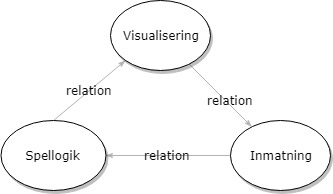
\includegraphics[width=0.5\textwidth, center]{System.jpg}
	\caption{Systemets tre objekt och deras relationer till varandra}
	\label{fig:System}
\end{figure}

Fördelar med denna struktur är att det är enklare att hitta fel i systemet och programkoden blir enklare att läsa då koden blir mer linjär och flödet är alltid riktat åt ett håll så som ses i \ref{fig:System}.

Visualiserings och spellogik objekten byggs upp i CryEngine 4 och skrivs i Lua. Inmatnings objekten kommer handskas både i CryEngine 4 och en arduino. På arduinon skrivs koden i C och kommer endast hantera de externa kontrollernas.  

\section{Standarder}
Det finns inga speciella standarder som behövs följas.

\section{Utvecklings-miljö}

I projektets utvecklingsfas kommer flera olika verktyg användas för att bygga och hantera slutprodukten. Dessa verktyg och dess användningsområde är samlade i tabell \ref{utvecklingsmiljö}. 


\begin{table}[H]
	\centering
	\caption{All programvara som används för att utveckla systemet}
	\label{utvecklingsmiljö}
	\begin{tabular}{ | p{9em} | m{6em} |p{23em}| } 
		\hline
		\textbf{Programtyp}&\textbf{Programnamn}  &\textbf{ Användningsområde} \\ 
		\hline
		Spelmotor &CryEngine 4 & Använd som grafikmotor och nivåskapare. \\ 
		\hline
		3D Modellering &3DS Max &Används till att skapa alla 3D modeller  \\ 
		\hline
		Bildbehandlings-program &Photoshop&Används till att skapa texturer  \\ 
		\hline
		Utvecklingsmiljö &Arduino Software &Används som utvecklingsmiljö när program skrivs till Arduinon  \\ 
		\hline
		Versionshantering &Git &Används till att hålla koll på tidigare versioner och underlätta samkodning  \\ 
		\hline
		Projekthantering &Hack n plan &Används till att hantera projektets olika delar och moment.  \\ 
		\hline

	\end{tabular}
\end{table}

Dessa programvaror skall användas av teamet, programvara till andra områden än de i tabell \ref{utvecklingsmiljö} får väljas av varje utvecklare.
	



\chapter{Projekthantering}

Olika projekthanteringsmetoder ger olika fördelar och nackdelar och en projekthanteringsmetod som passar projektet måste finnas.

\section{Utvecklingsmetodik}
Från kravspecifikationen som ses i bilaga \ref{Kravspecifikation} kan det ses att kunden inte har satt speciellt hårda krav på vad som slutprodukten skall innehålla vilket genererar att utvecklingsteamet har stor möjlighet att påverka vad innehållet kommer vara. Då bra idéer kan uppstå när som så är det bra och ha en utvecklingsmetodik som är flexibel. Därför har agil utveckling valts till detta projekt.

Agil utveckling kallas ofta för lättrörliga metoder eller iterativa metoder och menas att varje projekt bryts ner i mindre delar som kan utvecklas var för sig. Detta gör att det alltid finns fungerande programvara efter varje iteration. Inom agil utveckling följer man 4 st riktlinjer\cite{Sewell2012asd}:

\begin{itemize}
	\item Värderar individer och interaktion över processer och verktyg.
	\item Värderar fungerande programvara över omfattande dokumentation.
	\item Värderar kundsamarbeten över kontraktsförhandlingar.
	\item Värderar att svara på förändring över att följa en plan.
\end{itemize}
Detta kan sammanfattas med att agil utveckling är värdedrivande, det vill säga att utvecklingsteamet skall prioritera det som ger värde till slutprodukten.

Utvecklingsteamet kommer arbeta i små sprintar som är mellan 1-4 veckor långa. Under denna tiden går hela utvecklingsteamet igenom en full utvecklingscykel som involverar planering, krav analys, design, kodning, enhetstest\footnote{Enhetstest - Ett test som programmeraren själv skriver för att kolla sin kod.} och acceptanstest\footnote{Acceptanstest - Ett test där kunden granskar och ser att produkten följer kraven. }\cite{Sewell2012asd}. I slutet på varje sprint skall en hel funktionalitet vara implementerad. Detta sättet att jobba på ger att det alltid finns fungerande kod. 

En teknik som förespråkas inom agil utveckling är par programmering\cite{Sewell2012asd}. Par programmering går ut på att två programmerare sitter tillsammans och skriver kod. Den som skriver kallas föraren och den andra programmeraren kallas navigatören. Under tiden föraren skriver kod så granskar navigatören och pekar ut fel och ger råd till föraren. Detta genererar att fel kan upptäckas tidigt i processen och att koden blir mer läsbar direkt. Par programmering kommer att användas vid de viktigaste processerna så som koden för att kontrollera de externa kontrollerna. 

Inom agil utveckling förespråkas att så fort som möjligt ha en fungerande programvara för att sedan refaktorera den. Detta sätt kommer teamet jobba på för att säkerställa att det alltid finns något att leverera i slutet på varje sprint. Detta sätt ser ungefär ut som figur \ref{fig:refaktorering}.

\begin{figure}[h]
	\includegraphics[width=0.7\textwidth, center]{agil.png}
	\caption{Arbetsprocessen där fokus är på att ha färdig programvara.}
	\label{fig:refaktorering}
\end{figure}



\section{Organisation}


Detta projekt har tillgång till 10st utvecklare under 12 månaders tid för att färdigställa slutprodukten enligt kravspecifikationen i bilaga \ref{Kravspecifikation}. Förutom dessa 10st utvecklare så finns även en projektansvarig som är överst ansvarig för alla utvecklarna. 

Dessa 20st utvecklare är indelade i 2 grupper med olika arbetsuppgifter. Uppdelningen kan ses i tabell \ref{Utvecklare}.
\begin{table}[h]
	\centering
	\caption{Fördelningen mellan utvecklare i projektet och dess arbetsuppgifter}
	\label{Utvecklare}
	\begin{tabular}{ | p{10em} | m{3em} |p{23em}| } 
		\hline
		\textbf{Utvecklingsområde}&\textbf{Antal}  &\textbf{ Förklaring} \\ 
		\hline
		Spellogik &7st & Ansvarar för att all spellogik finns och att de externa kontrollerna fungerar med spelet. \\ 
		\hline
		Modellering och nivåeditering &3st & Ansvarar för att skapa alla 3D modeller och texturer till spelet. Sätter även ihop alla nivåer.  \\ 
		\hline
	
	\end{tabular}
\end{table}

I varje arbetsgrupp finns de tre roller scrummästare, produktägare och utvecklingsteam. Scrummästaren ansvar är att se till att alla rutiner och principer efterföljs och skall ses som en ledare över gruppen. Produktägaren skall se till att utvecklingen av produkten sker på ett sådant sätt att värdet maximeras för kunden och har även ansvar för backloggen\footnote{Backlogg - Är en lista över allt som skall komma in i den slutgiltiga produkten. Backloggen är dynmiskt och uppdateras. }. Utvecklingsteamet skall bestå av utvecklare med tillräcklig kompetens inom området för att kunna slutföra en sprint utan hjälp utifrån och skall vara självstyrande\cite{Scrumguiden}. 


Projektansvariga roll är att vara scrummästare och produktägare över alla utvecklingsteam för att säkerställa att alla teamen jobbar mot samma mål och att ingen del av teamen ligger efter.

\section{Tidsplan}
Detta projekt har ett tidsspann på 52 veckor för att få fram en slutprodukt enligt kravspecifikation i bilaga \ref{Kravspecifikation}. Projektet har en start i vecka 12 2018 och kommer att slutföras vecka 11 2019 då den slutgiltiga produkten skall visas upp för kunden. 

Arbetsgruppen kommer jobba inom något som kallas sprints där varje sprint är mellan 1-4 veckor. Till varje sprint diskuterar produktägaren och utvecklingsteamet om vad som skall göras under nästa sprint och längden på denna. Målet efter varje sprint är att kunna visa upp ett färdigt delsystem. 

För att ge frihet till utvecklingsteamet så har en grov tidsplan tagits fram som endast visar när vis funktionalitet skall vara implementerad och vad som sker mellan deadlines är det upp till produktägaren att se till att rätt saker sker.  Tidsplanen kan ses i figur \ref{fig:tidsplan}.

\begin{figure}[H]
	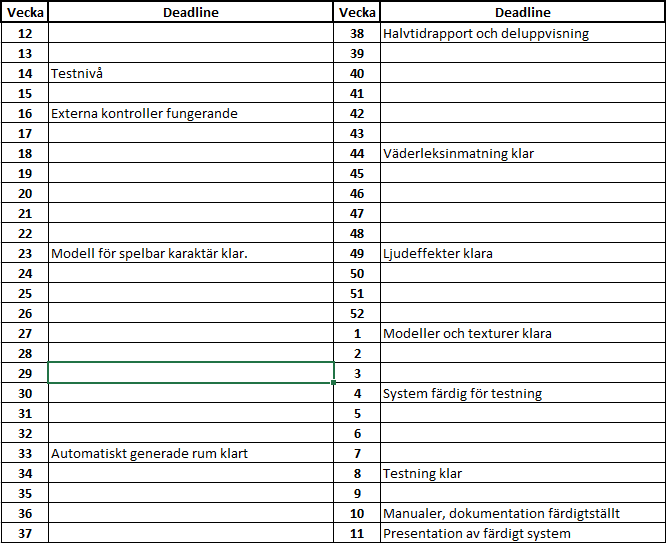
\includegraphics[width=0.7\textwidth, center]{tidsplan.jpg}
	\caption{Den grova tidsplanen för projektet.}
	\label{fig:tidsplan}
\end{figure}
Det faller mycket ansvar på produktägaren att se och bryta upp deadlines i poster så utvecklingsteamen har något att jobba mot.


\section{Milestones och leverabler}

\textcolor{red}{Mer detaljerad beskrivning och motivering av milestones och leverabler, såsom rapporter, prototyper
och färdigt system.
}


\chapter{Rutiner och principer}

För att öka produktiviteten och samarbetet mellan alla utvecklare sätts rutiner upp. Dessa skall hjälpa att all kod och dokument följer ett särskilt mönster så att det inte blir misskommunikation mellan utvecklare.

\section{Mötesprinciper och rutiner}

Det kommer ske tre olika sorters möten och de är veckomöte, sprintmöte och scrummöte.  

Veckomöte är ett möte som infaller varje måndag klockan 08:15 för att säkerställa att all vet vad de ska göra den kommande veckan samt att påminna om eventuella kundmöten. Detta mötet skall ta ungefär 30 min.

Under sprintmötet bestämts vad som skall ske under nästa sprint och vad som skall färdigställas. Arbetsuppgifter delas ut bland de ansvariga utvecklarna som sedan delar ut de till sina utvecklargrupper. Detta mötet är beräknat till ca 60 min.

Scrummöterna sker i varje utvecklingsgrupp och där tas problem upp och diskuteras hur långt alla har kommit med sprinten.  Detta mötet är beräknat till ungefär 5 min.

\section{Kravhantering och -sårning}
Kraven kommer hanteras i en backlogg som produktägaren i varje team ansvarar över. Alla krav i backloggen kommer att grupperas så det enkelt går att se vilka poster som tillhör vilket team samt vilka poster som påverkar alla. 

Alla poster kommer hanteras av verktyget hack n plan som har ett kanban\footnote{Kanban - Ett utryck från Japan där de satte upp en tavla med alla olika produkter och var de var i en process.} upplägg. I detta verktyg kan de ses vem som jobbar på projektet samt vilka poster som är var i processen. 

Projektansvarige har ansvarat att se till att kraven fortfarande är relevanta för kunde och att se till att kunden är med i processen och ser produkten i alla steg.

\section{Versionshantering, -system och rutiner}
Versionhantering är en viktigt pelare i ett projekt för att enklare kunna se vem som gjorde vad och gå tillbaka till gamla versioner. I detta projekt kommer Git användas som versionhanteringsprogram tillsammans med en extern server. Den externa serven kommer ligga på Gitlab. Valet att ha den externa servern på Gitlab grundar sig på tidigare licenser.

För att undvika konflikter och trasig kod så skall några få riktlinjer följas:
\begin{itemize}
	\item Alla commitments skall kommenteras kort. Nya tillägg skall kommenteras vad de gör och ändringar på gammal kod kommenteras vad de har ändrats. 
	\item Master branchen skall alltid innehålla fungerande kod, alla ändringar görs på en egen branch som sedan mergar in till mastern när den fungerar.
	\item Alla namn på branches skall innehålla i namnet vad som utvecklas och namn på ansvarig utvecklare. Stilen på namnet är \textit{Process\_Namn} och ett exempel kan se ut \textit{WrapperInput\_Daniel}.
	\item När en branch är fungerande skall alla test tas bort och branchen mergas in i mastern och sedan skall alltid branchen raderas om allt arbete på den är klar.
	\item Branches på branches behöver inte ha en ansvarig utvecklare i namnet. 
\end{itemize}

Dessa punkter är riktlinjer och skulle ett special dyka upp så skall detta diskuteras på ett möte.


\section{Arkitektur- och programdesign, standarder och rutiner}
All kod som skrivs skall följa tidigare uppsatta riktlinjer och för att se att all kod följer standarden kommer kod genomgångar ske. Kod genomgångarna sker genom att en utvecklare som inte har skrivit den specifika koden går in och läser och bedömer koden genom dessa riktlinjer:
  \begin{itemize}
  	\item Läsbarhet - Hur lätt koden är att läsa för en utomstående.
  	\item Struktur - Följer koden de strukturer som är uppsatta.
  	\item Välskriven - Är koden skriven på ett sätt som optimerar prestanda.
  	\item Dokumenterad - Är koden dokumenterad på rätt sätt.
  \end{itemize}
Om koden inte går igenom dessa krav får utvecklaren skriva om den för att sedan genomgå en ny kod genomgång.
\section{Dokumentationsprinciper och rutiner}
Dokumentation är en viktig del för att underlätta förståelse mellan utvecklare. Nedan beskrivs riktlinjerna för dokumentation.

\subsection{Programkod}
Programkod skall kommenteras på två olika ställen. En kommentar i toppen på varje fil och en över varje funktion. Kommentaren i toppen på varje fil skall innehålla:
\begin{itemize}
	\item Namnet på ansvarig utvecklare. Det menas med utvecklaren som är ansvarig för området och inte utvecklaren som har skrivit koden.
	\item Eventuella licenser
	\item Evuentuella tredjeparts-APIer som används.
	\item Kort sammanfattning vad filen gör.
\end{itemize}
All kommentering skall ske i Engelska.
\subsection{Möten}
Alla veckomöten skall dokumenteras enligt en fördefinerad mall som kan ses i bilaga \ref{protokoll}. De dagliga scrum mötena dokumenteras kortfattat i en textfil som lägg på samma server som all kod och hanteras av git. All dokumentation från möten sker på svenska.
\subsection{Slutproduktion}
Slutprodukten som är ett spel kommer dokumenteras på två sätt. En dokumentation kommer ske direkt i spelet iform av en introduktion till spelet och den andra dokumentationen är en manual hur slutprodukten skall kopplas samman. 

Indroduktionen i spelet kommer skrivas direkt i Unity3D och skall fokusera på att ge en grafisk handledning istället för text. Informationen ges på de språket som användaren har valt att spela i.

Manualen kommer skrivas i Latex och kommer innehålla en stegvis beskrivning på hur alla tillbehör sätt tillsammans samt hur slutprodukten installeras. Felsökning kommer även inkluderas i manualen. Manualen skrivs på Engelska.

\section{Kvalitetssäkring}
För att säkerställa att all funktionalitet fungerar som den skall så sker det flera olika tester på olika stadier. Varje enskild programmerare kommer sköta egna enhetstest för att prova sin programkod. 

Vid de fallen där flera olika moduler samarbetar kommer ett integrationstest ske, detta kommer att göras av utvecklare som inte har utvecklad den delen som skall testas. Går det inte att få utvecklare som har skrivit koden att göra testet så tas de utvecklare som har minst överblickande koll på koden. Detta är för att testen inte ska skrivas av vana ögon utan testen skall prova saker som utvecklarna kanske inte har tänkt på.

Under hela processen kommer systemtest ske för att se till att all integration tillsammans fungerar.

Ingen CI-server kommer användas då uppsättningen är tidsödslande samt funktionalitet som en CI-server ger detta projekt är minimal.


\chapter{Analys och diskussion}

När en arbetprocess är vald är det viktigt att analysera vilka fallgroppar det kan finnas.


\section{Resultat}
Valet att hyra in en spelmotor är ett val som är väldigt lättmotiverat men valet av viken spelmotor är lite mer diffus. Valet denna gång grundade sig i hur stor del av vinsten som skulle gått till företaget som utvecklade spelmotorn men det betyder inte att det kommer varit det bästa valet. Det är svårt att förutspå inlärningskurvan för utvecklarna till exempel. Valet mellan CryEngine 4 och Unreal Engine 4 grundar sig enbart på den ekonomiska aspekten.

Att använda refaktorering istället för planering är ett resultat som inte var väntat men då kraven från kunden är väldigt fria gällande innehåll i slutprodukten så är det bra och inte knyta fast en plan för hela projektet från början. Projektet går fortare om teamet försöker få något som fungerar först istället för att göra ordentligt från början. Till exempel om det tar lång tid innan de externa kontrollerna fungerar så kommer teamet inte kunna prova spelet på riktigt innan det är klart.

\section{Arbetet i ett vidare sammanhang}

Då slutprodukten skall vara riktad mot barn så är det viktigt att det finns en tanke bakom allt som finns i produkten. Barn är väldigt lättpåverkade och handlingar i ett spel kan påverka deras syn på världen. Därför är det viktigt att ha ett fokus på lärande, samarbete och förståelse. Ett exempel är att barnen får en positiv effekt att göra något som inte är tillåten så som att de måste trycka på en knapp som det står "tryck ej" på för att komma vidare. Detta leder till att barnen tror att det är okej att trycka på sådana knappar.


\chapter{Slutsatser}
Systemets arkitektur bestämdes till MVC vilken genererar en mer linjär process som kommer underlätta utvecklingen och felsökningen mellan de olika delarna.

Valet att hyra in en spelmotor visade sig väldigt självklart ur ett ekonomiskt synvilken då flertalet av de analyserade spelmotorerna var väldigt billiga i utvecklingsammanhanget och visa var också gratis. När det kom till hur stor del av avkastningen från produkten de skulle ha så skillde det sig en del och det var där som CryEngine stod ut. 

Det visade sig att de flesta spelmotorer hade stöd för externa kontroller via en microkontroller. Detta grundar sig mycket i att de flesta av spelmotorerna har öppen källkod så det finns alltid en möjlighet att skriva egna koder som fixar funktioner som saknas från grunden i spelmotorn.

Det fanns många skäl till att använda refaktorering istället för planering. Främst är det att projektet blir mer redundant och det ger utvecklarna större möjligheter att komma med egna förslag på förändringar i slutprodukten.



\bibliographystyle{vancouver}
\bibliography{referenser}

\addcontentsline{toc}{chapter}{Litteraturförteckning}

\pagestyle{empty}

\appendix

\chapter{Kravspecifikation}\label{Kravspecifikation}
\begin{table}[H]
	\centering
	
	\begin{tabular}{ | m{5em} | m{30em}| } 
		\hline
		Krav nr 1& Systemet skall minst använda sig av 3 externa knappar och 1 extern spak.   \\ 
		\hline
		Krav nr 2 & Systemet skall vara engagerande.  \\ 
		\hline
		Krav nr 3 & Systemet skall kunna brukas av en sexåring. \\ 
		\hline
		Krav nr 4& Systemet skall kräva minst två spelare för att vara spelbart. \\ 
		\hline
		Krav nr 5 & Systemet skall inte ge negativ respons vid fel utan ge konstruktiv kritik till användaren. \\ 
		\hline
		Krav nr 6 & Systemet skall inte innehålla ett traditionellt poängsystem. \\ 
		\hline
		Krav nr 7& En användare skall kunna lära sig kontrollerna för systemet under 2 minuter. \\ 
		\hline
		Krav nr 8 & Systemet skall öka svårighetsgrader så att det är svårt att bemästra systemet. \\ 
		\hline
		Krav nr 9 & Systemets skall ha rymd eller programmeringstema. \\ 
		\hline
		Krav nr 10& Systemet får inte manipulera projektionsvägen. \\ 
		\hline
		Krav nr 11& Systemet skall använda grafiska hjälpmedel för att visa knappar och spakars funktionalitet.  \\ 
		\hline
		Krav nr 12& Systemet skall gå att montera för en normalteknisk person på ca 2h. \\ 
		\hline
		Krav nr 13& Systemet skall kunna användas dagligen under 2 år utan att behöva repareras \\ 
		\hline
		Krav nr 14 & Systemet skall kunna skalas om till rum i olika storlekar. Minsta storlek på rum är 2x2 meter. \\ 
		\hline
	\end{tabular}
	\caption{Kravspecifikationen som projektet skall uppfylla}

\end{table}


\chapter{Protokoll mall}\label{protokoll}


\end{document}